\section{Основи багатопотоковості}

\subsection{Мета:}
ознайомитися з поняттям потоку, класами та методами, які реалізують роботу потоків;
познайомитися з особливостями реалізації багатопотоковості в JavaFX; клас ProgressBarTableCell (Індикатор прогресу)

\subsection{Теоретичний матеріал}

\begin{enumerate}
	\item Поняття багатопотоковості
	\item Прості методи класу Thread
	\item Способи створення потоків. Методи опрацювання.
	\item Стани потоків. Планувальник черги.
	\item Синхронізація потоків.
	\item Інтерфейси Callable та Future.
\end{enumerate}

\subsection{Проект «Послідовність Фібоначчі»}

Розробити проект, в якому за заданим порядковим номером виводиться число Фібоначчі (Рис.~\ref{fig:image1}).

\begin{figure}[h]
	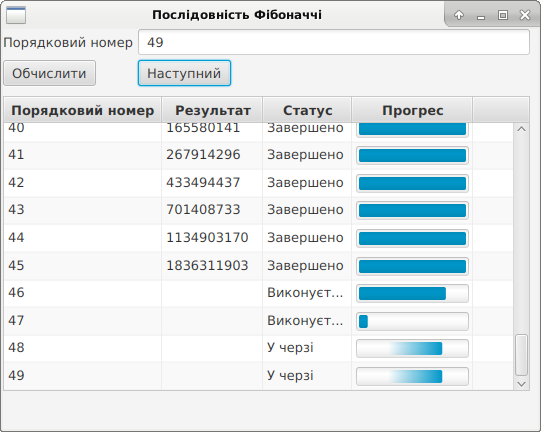
\includegraphics{chapter21/images/image1.png}
	\caption{}
	\label{fig:image1}
\end{figure}

\paragraph{Завдання:}
\begin{itemize}
	\item Створення графічного інтерфейсу для введення та виведення інформації.
	\item Написати метод обчислення числа Фібоначчі.
	\item Винести обчислення до окремого потоку
	\item До графічного інтерфейсу додати елементи візуалізації роботи потоків
\end{itemize}

\paragraph{Хід роботи:}
\begin{enumerate}
	\item Створюємо проект JavaFX (файл Fibonacci.fxml, та його контролер – FibonacciController).

	\item Використовуючи Scene Builder створюємо графічний інтерфейс програми з текстовим полем, написом для виведення результату і кнопкою (Рис.~\ref{fig:image2})
\begin{figure}[h]
	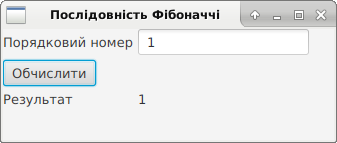
\includegraphics{chapter21/images/image2.png}
	\caption{}
	\label{fig:image2}
\end{figure}

	\item Задаємо значення параметрів для елементів керування (для текстового поля fx:id – input, для кнопки onAction – alculate для результату fx:id - result) і додаємо їх у контролер.

	\item В обробнику calculate реалізовуємо обчислення числа Фібоначчі за введеним порядковим номером. Перевіряємо роботу програми.

	Щоб не доводилось використовувати для перевірки дуже великі числа, можна штучно сповільнити алгоритм, додавши у нього пустий цикл
	\mintinline{java}{for (long j=0; j<100000000; j++);}

\begin{minted}{java}
public class FibonacciController {
	@FXML TextField input;
	@FXML Label result;
	@FXML
	public void calculate() {
		long n = Long.parseLong(input.getText());
		long a = 0, b = 0, c = 1;
		for (int i = 0; i<n; i++) {
			a = b;
			b = c;
			c = a + b;
			for (long j=0; j<100000000; j++);
		}
		result.setText(Long.toString(c));
	}
}
\end{minted}

Тепер можна побачити, що до завершення обчислень інтерфейс програми повністю блокується. 
Це відбувається тому, що вся програма JavaFX виконується в одному потоці. Отже, усі тривалі операції (складні обчислення, завантаження великого файлу) потрібно виносити з головного потоку програми. Але компоненти JavaFX не пристосовані до спільного доступу (non thread safe) і безпечно працювати з ними можна тільки з головного потоку. Реалізація такого доступу стандартними методами Java є складною і тому у склад JavaFX входить пакет javafx.concurrent з класами, що полегшують цю задачу. Основним з цих класів є клас Task. 

	\item Створюємо клас FibonacciTask, який наслідує клас Task, та пишемо реалізацію методу call().

	При наслідуванні класу Task вказується тип результату. В даному випадку це Long. Вхідні параметри передаються через конструктор класу. Обчислення числа Фібоначчі переносимо з контролера у метод call() і результат обчислень просто повертається з нього через оператор return.

\begin{minted}{java}
public class FibonacciTask extends Task<Long> {
	private final long n;
	public FibonacciTask(long n) {
		this.n = n;
	}
	@Override
	protected Long call() throws Exception {
		long a = 0, b = 0, c = 1;
		for (long i = 0; i<n; i++) {
			a = b;
			b = c;
			c = a + b;
			for (long j=0; j<100000000; j++);
		}
		return c;
	}
}
\end{minted}

	\item Змінюємо контролер (даний пункт не обов'язковий, але якщо учні знайомі з лямбда-виразами, то він є більш універсальним, бо в такому випадку в обробнику події можна виконувати будь-які події, наприклад, записувати результати у файл. Є ще один метод взаємодії задачі з головним потоком через метод runLater().)

\begin{minted}{java}
public class FibonacciController {
	@FXML TextField input;
	@FXML Label result;
	@FXML
	public void calculate() {
		long n = Long.parseLong(input.getText());
		FibonacciTask task = new FibonacciTask(n);
		task.setOnSucceeded((succeeded Event) -> {
			result.setText(task.getValue().toString());
		});
        Thread thread = new Thread(task);
        thread.setDaemon(true);
        thread.start();
	}
}
\end{minted}

Як видно з коду при натисканні на кнопку спочатку створюється об'єкт класу FibonacciTask і в конструктор передається порядковий номер елемента послідовності. Потім прив'язується обробник до події onSucceeded, який буде виконано після завершення задачі. Всередині обробника зчитується результат виконання задачі через метод task.getValue(), конвертується в рядок (оскільки дана задача повертає значення типу Long) і записується в мітку result.
Після задання параметрів задачі створюється об'єкт класу Thread (з стандартної бібліотеки Java). Задання параметру thread.setDaemon(true); потрібне щоб незавершений потік не блокував закриття всієї програми (по замовчуванню перед виходом програма чекає завершення всіх своїх потоків). І далі задача запускається на виконання в окремому потоці через метод thread.start().

	\item Запустимо програму на виконання.
Обчислення більше не заморожує інтерфейс користувача. Можна навіть обчислювати кілька значень паралельно, швидко вводячи число в поле і натискаючи кнопку. Але оскільки всі задачі записують результат у той самий елемент форми - то нові значення перезаписують старі. 

	\item Створимо таблицю (TableView, fx:id - resultTable) з одним стовпцем (fx:id значення resultCol) для виведення результатів обчислення (Замінюємо мітку Label). (Рис.~\ref{fig:image3})
	
	\begin{figure}[h]
		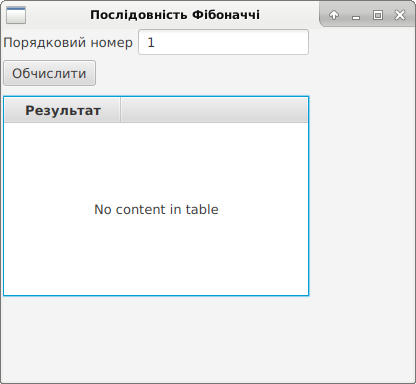
\includegraphics{chapter21/images/image3.png}
		\caption{}
		\label{fig:image3}
	\end{figure}

	\item Додаємо у контролер таблицю та стовпець у такому вигляді
\begin{minted}{java}
@FXML TableView<FibonacciTask> resultTable;
@FXML TableColumn<FibonacciTask, Long> resultCol;
\end{minted}
Такий опис вказує, що таблиця призначена для відображення об'єктів класу FibonacciTask. А у стовпці буде виводитись значення типу Long (при виведенні воно автоматично перетвориться в рядок з використанням стандартного методу toString для цілих чисел).

	\item Додаємо метод initialize(){} та змінюємо метод  calculate().

	Завдяки тому, що результат є властивістю (property) класу Task, то найпростіший спосіб вивести його через прив'язку (при зміні значення одного параметру змінюється значення зв'язаного з ним параметру). В TableView можна буде спостерігати за значенням результату result (воно буде оновлюватись автоматично). Для цього треба тільки встановити відповідність між властивістю класу та стовпцем таблиці використовуючи метод setCellValueFactory. Ця прив'язка буде виконуватись одразу при відкритті вікна у методі initialize.

	При такому підході обробник події більше не потрібен і об'єкт task можна просто додати в таблицю перед запуском потоку.

\begin{minted}{java}
public class FibonacciController {
	@FXML TextField input;
	@FXML Label result;
	@FXML TableView<FibonacciTask>resultTable;
	@FXML TableColumn<FibonacciTask, Long>resultCol;
	@FXML
	public void initialize() {
		resultCol.setCellValueFactory(new PropertyValueFactory<FibonacciTask, Long>("value"));
	}
	@FXML
	public void calculate() {
		longn = Long.parseLong(input.getText());
		FibonacciTask task = new FibonacciTask(n);
		resultTable.getItems().add(task);
		Thread thread = new Thread(task);
		thread.setDaemon(true);
		thread.start();
	}
}
\end{minted}

	Тепер при натисканні на кнопку у таблицю одразу додається новий рядок, а коли задача поверне результат обчислень - то він автоматично виводиться у відповідну клітинку.

	\item Додаємо, для зручності перевірки, кнопку, при натисканні на неї буде збільшуватися значення у полі input на одиницю і одразу запускатися метод calculate(). (Рис.~\ref{fig:image4})

	\begin{figure}[h]
		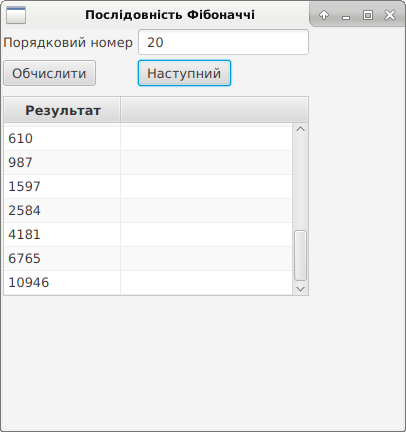
\includegraphics{chapter21/images/image4.png}
		\caption{}
		\label{fig:image4}
	\end{figure}

	\item Додаємо в таблицю стовпці Результат та Статус, виконуємо прив’язку параметрів задачі до цих стовпців і в середині задачі додаємо оновлення статусу і заголовку задачі (Рис.~\ref{fig:image5}).

	\begin{figure}[h]
		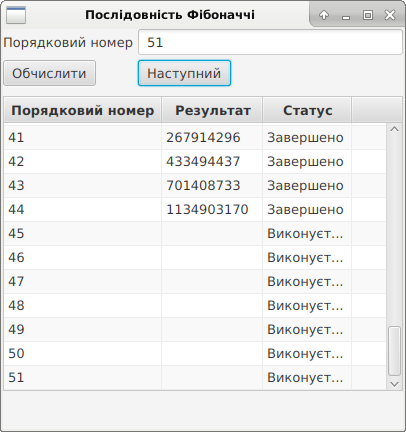
\includegraphics{chapter21/images/image5.png}
		\caption{}
		\label{fig:image5}
	\end{figure}

	Клас Task має інші параметри крім value, який зберігає результат виконання. Використовуючи параметр title, відобразимо в таблиці порядковий номер числа Фібоначчі, яке в даний момент обчислюється в задачі. Всередині класу FibonacciTask його можна змінювати за допомогою методу updateTitle (цей параметр має рядковий тип, тому число потрібно сконвертувати). Прив'язка параметру title до стовпця таблиці відбувається по аналогії до value.

	Ще один параметр класу Task – message, який можна використовувати для передачі текстових повідомлень в головний процес. 

	Додамо в таблицю стовпець statusCol, а всередині класу FibonacciTask методом updateMessage будемо відображати користувачу статус виконання задачі.

	\item Додаємо стовпчик Прогрес до таблиці, який буде відображати індикацію прогресу у вигляді числа.

	Останній зі стандартних параметрів класу Task це progress – дійсне число в межах від 0 до 1, в якому задача може передавати відсоток своєї завершеності. Метод updateProgress дещо відрізняється від аналогічних для решти параметрів. У нього передаються два числа (цілі або дійсні), де перше вказує на кількість завершених дій, а друге – загальну кількість дій, які необхідно виконати. Наприклад, при завантаженні файлу з мережі у другому параметрі можна передавати загальний розмір файлу, а в першому – кількість вже завантажених байтів. Приведення параметру progress до потрібних меж буде виконано автоматично.

	\item Модифікуємо метод call так, щоб updateProgress викликався на кожній ітерації циклу. 
В контролері прив'язуємо параметр progress до нового стовпця таблиці методом setCellValueFactory. Якщо запустити програму тепер, то прогрес буде виводитись у вигляді дійсного числа. 

	\begin{figure}[h]
		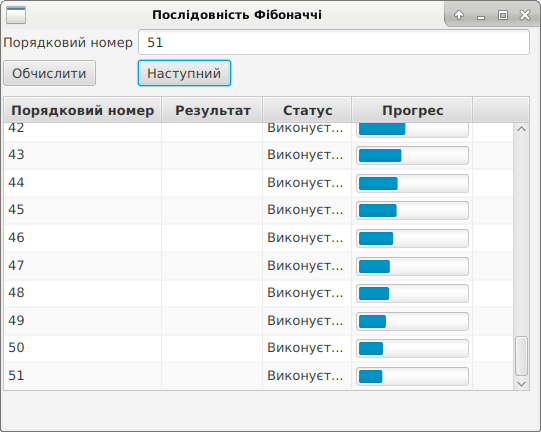
\includegraphics{chapter21/images/image6.png}
		\caption{}
		\label{fig:image6}
	\end{figure}

	\item Змінюємо представлення індикатора прогресу з числового на графічний (Рис.~\ref{fig:image6}).
Для більшої наочності можна відображати його у вигляді елементу ProgressBarTableCell (спеціальний індикатор прогресу, розрахований на відображення в TableView). Для його прив'язки використовується метод setCellFactory. Результуючий код контролера і задачі.

\begin{minted}{java}
package application;

import javafx.fxml.FXML;
import javafx.scene.control.TextField;
import javafx.scene.control.cell.ProgressBarTableCell;
import javafx.scene.control.cell.PropertyValueFactory;
import javafx.scene.control.Label;
import javafx.scene.control.TableView;
import javafx.scene.control.TableColumn;
public class FibonacciController {
	@FXML TextField input;
	@FXML Label result;
	@FXML TableView<FibonacciTask> resultTable;
	@FXML TableColumn<FibonacciTask, Long> resultCol;
	@FXML TableColumn<FibonacciTask, String> titleCol;
	@FXML TableColumn<FibonacciTask, String> statusCol;
	@FXML TableColumn<FibonacciTask, Double> progressCol;
	@FXML
	public void initialize() {
		resultCol.setCellValueFactory(new PropertyValueFactory<FibonacciTask, Long>("value"));
		titleCol.setCellValueFactory(new PropertyValueFactory<FibonacciTask, String>("title"));
		statusCol.setCellValueFactory(new PropertyValueFactory<FibonacciTask, String>("message"));
		progressCol.setCellValueFactory(new PropertyValueFactory<FibonacciTask, Double>("progress"));
		progressCol.setCellFactory(ProgressBarTableCell.<FibonacciTask>forTableColumn());
	}
	@FXML
	public void calculate() {
		long n = Long.parseLong(input.getText());
		FibonacciTask task = new FibonacciTask(n);
		resultTable.getItems().add(task);
		Thread thread = new Thread(task);
		thread.setDaemon(true);
		thread.start();
	}
	@FXML
	public void next() {
		long n = Long.parseLong(input.getText());
		n++;
		input.setText(Long.toString(n));
		calculate();
	}

}
\end{minted}

\begin{minted}{java}
package application;

import javafx.concurrent.Task;
public class FibonacciTask extends Task<Long> {
	private final long n;
	public FibonacciTask(long n) {
		this.n = n;
		updateTitle(Long.toString(n));
		updateMessage("У черзі");
	}
	@Override
	protected Long call() throws Exception {
		updateMessage("Виконується");
		long a = 0, b = 0, c = 1;
		for (long i = 0; i < n; i++) {
			a = b;
			b = c;
			c = a + b;
			for (long j = 0; j < 100000000; j++);
			updateProgress(i, n-1);
		}
		updateMessage("Завершено");
		return c;
	}
}
\end{minted}

	\item Обмежуємо кількість паралельних потоків за допомогою планувальника.

	Тепер видно, що скільки б задач ми не запускали, всі вони виконуються паралельно. Але комп'ютер має обмежену кількість ядер, тому при великій кількості потоків операційна система просто періодично перемикається між ними, а швидкодія від цього не зростає. Постійне створення та знищення потоків ще більше сповільнює виконання. Отже, замість того, щоб створювати потік на кожну задачу, можна скористатись класом java.util.concurrent.ExecutorService, який призначений для автоматичного керування потоками. А саме – використаємо його реалізацію fixedThreadPool. Цей клас створює фіксовану кількість потоків і по черзі виконує всі поставлені в чергу задачі.

	Для створення об'єкту використовуємо метод
\begin{minted}{java}
ExecutorService executor = Executors.newFixedThreadPool(2);
\end{minted}
	параметр вказує кількість потоків, які буде запущено. А постановка задачі в чергу виконується командою \mintinline{java}{executor.execute(task);}

\begin{minted}{java}
package application;

import java.util.concurrent.ExecutorService;
import java.util.concurrent.Executors;
import javafx.fxml.FXML;
import javafx.scene.control.TextField;
import javafx.scene.control.cell.ProgressBarTableCell;
import javafx.scene.control.cell.PropertyValueFactory;
import javafx.scene.control.Label;
import javafx.scene.control.TableView;
import javafx.scene.control.TableColumn;

public class FibonacciController {
	@FXML TextField input;
	@FXML Label result;
	@FXML TableView<FibonacciTask> resultTable;
	@FXML TableColumn<FibonacciTask, Long> resultCol;
	@FXML TableColumn<FibonacciTask, String> titleCol;
	@FXML TableColumn<FibonacciTask, String> statusCol;
	@FXML TableColumn<FibonacciTask, Double> progressCol;
	ExecutorService executor = Executors.newFixedThreadPool(2);
	@FXML
	public void initialize() {
		resultCol.setCellValueFactory(new PropertyValueFactory<FibonacciTask, Long>("value"));
		titleCol.setCellValueFactory(new PropertyValueFactory<FibonacciTask, String>("title"));
		statusCol.setCellValueFactory(new PropertyValueFactory<FibonacciTask, String>("message"));
		progressCol.setCellValueFactory(new PropertyValueFactory<FibonacciTask, Double>("progress"));
		progressCol.setCellFactory(ProgressBarTableCell.<FibonacciTask>forTableColumn());
	}

	@FXML
	public void calculate() {
		long n = Long.parseLong(input.getText());
		FibonacciTask task = new FibonacciTask(n);
		resultTable.getItems().add(task);
		executor.execute(task);
	}

	@FXML
	public void next() {
		long n = Long.parseLong(input.getText());
		n++;
		input.setText(Long.toString(n));
		calculate();
	}

}
\end{minted}

	У цьому варіанті програми виконується не більше двох задач одночасно. Інші очікують своєї черги.

	Кінцевий вигляд вікна програми (Рис.~\ref{fig:image1}) та орієнтовне використання елементів для відображення інформації (Рис.~\ref{fig:image7})
	
	\begin{figure}[h]
		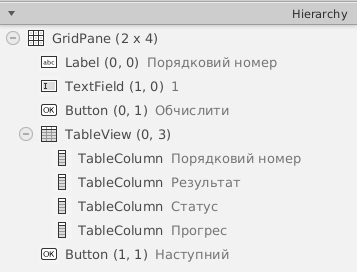
\includegraphics{chapter21/images/image7.png}
		\caption{}
		\label{fig:image7}
	\end{figure}
	
\end{enumerate}

\subsection{Задачі для самостійного виконання}
Реалізувати проект виводу простих дільників довільного числа, заданого користувачем. Обчислення дільників вивести в окремий потік, вивід дільників у таблицю виконувати по мірі знаходження (результат  задачі можна обновлювати через метод updateValue()).